%------------------------------------------------------------------------------
% Author(s):
% Varaun Ramgoolie
%
% Copyright:
%  Copyright (C) 2020 Brad Bachu, Arjun Mohammed, Varaun Ramgoolie, Nicholas Sammy
%
%  This file is part of Applied-Mathematics-Unit2 and is distributed under the
%  terms of the MIT License. See the LICENSE file for details.
%
%  Description:
%     Year: 2011
%     Module: 3
%     Question: 5
%------------------------------------------------------------------------------

%------------------------------------------------------------------------------
% 5 a
%------------------------------------------------------------------------------

\begin{subquestions}
	
\subquestion
We ae given a car which accelerates uniformly up an inclined plane.

\begin{subsubquestions}
	
\subsubquestion

\textbf{\textit{Simplify and Diagram:}} \\ \\
\begin{figure}[H]
	\begin{center}
		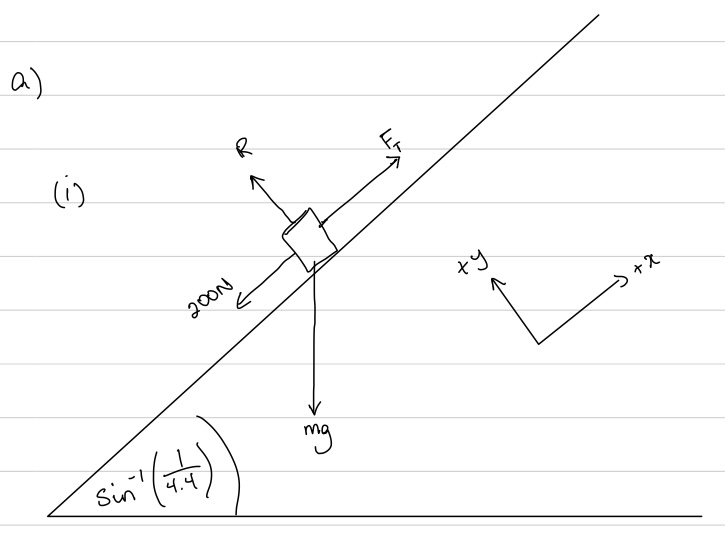
\includegraphics[scale=0.25]{../2011/figures/2011q5-1}
		\caption{\label{2011:q5:Diagram1} Diagram of forces on car.}
	\end{center}
\end{figure}
	
%------------------------------------------------------------------------------

\subsubquestion

\textbf{\textit{Simplify and Diagram:}} \\ \\
We can consider \rfig{2011:q5:Diagram1}. We are given the initial and final velocities of the car, together with the displacement of the car. By using our equations of motion, we can solve for the acceleration.




\textbf{\textit{Represent Mathematically:}} \\ \\
We will use the equation,
\begin{align}
	v^2 & = u^2 + 2as \nn \\
	\implies a & = \frac{v^2-u^2}{2s} \,.	
\end{align}




\textbf{\textit{Solve and Evaluate:}} \\ \\
By substituting our values, we get,
\begin{align}
	a & = \frac{(72kmh^{-1})^2-(54kmh^{-1})^2}{2(175m)} \nn \\
	  & = \frac{\left(\frac{72\times 1000}{3600}\right)^2-\left(\frac{54\times 1000}{3600}\right)^2}{2(175)} \nn \\
	  & = \frac{400-225}{350} \nn \\
	  & = 0.5ms^{-2} 
\end{align}

%------------------------------------------------------------------------------

\subsubquestion

\textbf{\textit{Simplify and Diagram:}} \\ \\
We can consider \rfig{2011:q5:Diagram1}. We will define the following forces as,
\begin{itemize}
	\item $\vec{W}$ which is the weight of the car,
	\item $\vec{R}$ which is the resistive forces on the car,
	\item $\vec{F_T}$ which is the tractive force of the car,
	\item $\vec{N}$ which is the normal reaction force of the car.
\end{itemize}
We will assume that there are no other forces acting on the car. As we are given that the car has a uniform acceleration, it is implied that there is a constant resultant force in the direction of the acceleration (+$x$ direction). By using Newton's Second Law, we can find the magnitude of this resultant force and thus, solve for the tractive force.



\textbf{\textit{Represent Mathematically:}} \\ \\
We will first resolve the forces into their components as,
\begin{align}
	\vec{W} & = -|\vec{W}|\cos\left({\arcsin\left(\frac{1}{4.4}\right)}\right)\yhat-|\vec{W}|\sin\left({\arcsin\left(\frac{1}{4.4}\right)}\right)\xhat \nn \\
	        & = -mg\cos\left({\arcsin\left(\frac{1}{4.4}\right)}\right)\yhat-\frac{1}{4.4}mg\xhat \\ \nn \\
	\vec{R} & = -|\vec{R}|\xhat \nn \\
	        & = -200 \xhat \\ \nn \\
	\vec{F_T} & = |\vec{F_T}|\xhat \\ \nn \\
	\vec{N} & = |\vec{N}|\yhat \,.
\end{align}

By Newton's Second Law, the resultant force in the $x$ direction, $F$, is,
\begin{equation}
	F = \sum F_x = ma_x \,, \label{2011:q5:Newt1}
\end{equation}
where $F_x$ represents the components acting in the $x$ direction and $a_x$ is the acceleration in the $x$ direction.




\textbf{\textit{Solve and Evaluate:}} \nn \\
By substituting our values into \req{2011:q5:Newt1}, we get,
\begin{align}
	\sum F_x & = ma_x \nn \\
	-\frac{1}{4.4}mg-200+|\vec{F_T}| & = ma_x \nn \\
	|\vec{F_T}| & = ma_x +\frac{1}{4.4}mg+200 \nn \\
	            & = (1100)(0.5)+\frac{1}{4.4}(1100)(10)+200 \nn \\
	            & = 3250 \,.
\end{align}

%------------------------------------------------------------------------------

\subsubquestion

\textbf{\textit{Simplify and Diagram:}} \\ \\
We can consider \rfig{2011:q5:Diagram1}. We can use our relationship between tractive force and power to find the maximum power generated.




\textbf{\textit{Represent Mathematically:}} \\ \\
We know that,
\begin{align}
	F_T & = \frac{\text{Power, P}}{\text{Velocity, v}} \nn \\
	\implies P_{\text{max}} & = F_T \times v_{\text{max}} \,.
\end{align}




\textbf{\textit{Solve and Evaluate:}} \\ \\
By substituting $F_T=3250$N and $v_{\text{max}}=20$ms$^{-1}$, we get,
\begin{align}
	P_{\text{max}} & = 3250 \times 20 \nn \\
	               & = 65000W = 65kW \,.
\end{align}
	
\end{subsubquestions}	
	
%------------------------------------------------------------------------------
% 5 b
%------------------------------------------------------------------------------
	
\subquestion
We are given two masses which are connected by a string over a smooth, weightless pulley.

\begin{subsubquestions}
	
	\subsubquestion
	
	\textbf{\textit{Sketch and Translate:}} \\ \\
	\begin{figure}[H]
		\begin{center}
			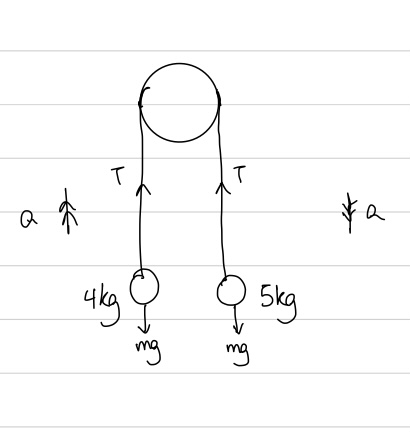
\includegraphics[scale=0.25]{../2011/figures/2011q5-2}
			\caption{\label{2011:q5:Sketch2} Pulley System.}
		\end{center}
	\end{figure}	
	We are asked to find the acceleration of the system given. This problem is a classic pulley problem and so, we should think about what we know about tension and forces in the context of pulleys.
	
	
	
	
	\textbf{\textit{Simplify and Diagram:}} \\ \\
	\begin{figure}[H]
		\begin{center}
			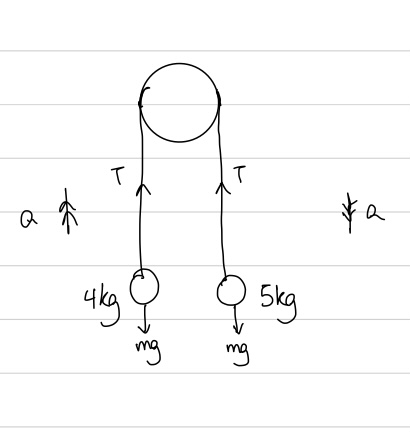
\includegraphics[scale=0.25]{../2011/figures/2011q5-2}
			\caption{\label{2011:q5:Diagram2} All forces on Pulley System.}
		\end{center}
	\end{figure}
	We will assume that both bodies move in only 1 dimension and that they behave as point particles. We will also assume that the mass of the string is 0 and inextensible. Thus, we know that the speed (and the magnitude of the acceleration) of both particles must be the same. Since the pulley is smooth, no energy is lost to friction. We should consider how the forces act on the different weights and motivate our solution from there.
	
	
	
	
	\textbf{\textit{Represent Mathematically:}} \\ \\ 
	Let us denote the displacements of the 5kg and 4kg masses so be $y_1$ and $y_2$ respectively. As the string is inextensible, we know that,
	\begin{align}
		y_1 & = -y_2 \nn \\
		\implies \ddd{y_1}{t} & = -\ddd{y_2}{t} \nn \\
		\implies \ddd{^2y_1}{t^2} & = -\ddd{^2y_2}{t^2} \nn \\
		a_1 & = -a_2 \,.
	\end{align}
	
	Let us first consider the forces on the 4kg mass. From Newton's 2nd Law, we get that,
	\begin{align}
		\sum F & = ma_1 \nn \\
		mg - T & = ma_1 \,.
	\end{align}
	
	Let us then consider the forces on the 5kg mass. From Newton's 2nd Law, we get that,
	\begin{align}
		\sum F & = ma_2 \nn \\
		mg-T & = ma_2 \,.
	\end{align}
	
	
	
	
	\textbf{\textit{Solve and Evaluate:}} \\ \\
	On the 5kg mass, we see that,
	\begin{align}
		mg - T & = ma_1 \nn \\
		\implies 5g-T & = 5a_1 \,. \label{2011:q5:PulleyEq1}
	\end{align}
	
	On the 4kg mass, we see that,
	\begin{align}
		mg - T & = ma_2 \nn \\
		\implies 4g-T & = 4a_2 \nn \\
		\implies 4g-T & = -4a_1 \nn \\
		T-4g & = 4a_1 \,. \label{2011:q5:PulleyEq2}
	\end{align}
	
	By solving \req{2011:q5:PulleyEq1} and \req{2011:q5:PulleyEq2} simultaneously, we get,
	\begin{align}
		\text{(\req{2011:q5:PulleyEq1}+\req{2011:q5:PulleyEq2}):} (5g-T)+[T-4g] & = (5a_1)+[4a_1] \nn \\
		g & = 9a_1 \nn \\
		\implies a_1 & = a = \frac{g}{9} = 1.11\text{ms}^{-2} \,.
	\end{align}
	
	%------------------------------------------------------------------------------
	
	\subsubquestion
	
	\textbf{\textit{Solve and Evaluate:}} \\ \\
	We can find the tension on the string by substituting our value from (a)(i) into \req{2011:q5:PulleyEq2}. We get,
	\begin{align}
		T-4g & = 4a_1 \nn \\
		T & = 4a_1 + 4g \nn \\
		& = 4\left(1.11 \right) + 40 \nn \\
		& = 44.44N \,.
	\end{align}

\end{subsubquestions}

\end{subquestions}